\begin{definition}
A \emph{concept} in CML represents anything
that has a coherent, cohesive meaning in a domain.
On the ER \cite{er} metamodel,
it corresponds to an \emph{entity};
in UML \cite{uml},
to a \emph{class}.
The CML \emph{concept} differs, however, from the UML \emph{class},
because it has only \emph{properties} (\ref{sec:properties}),
while the UML \emph{class} may also have \emph{operations}.
\end{definition}

\begin{examples}
Figure \ref{fig:ex:concepts} presents some examples of \emph{concepts} declared in CML.
As shown in the examples,
a \emph{concept} may have zero or more \emph{properties}
(\ref{sec:properties}),
and a \emph{property} may optionally declare a \emph{type}
(\ref{sec:primitive-types}, \ref{sec:collection-types}).
Also, as shown in the last example of figure \ref{fig:ex:concepts},
a \emph{concept} may specialize
(\ref{sec:generalization})
another \emph{concept}.
\end{examples}

\begin{figure}
\verbatimfont{\small}
\begin{framed}
\verbatiminput{examples/concepts.cml}
\end{framed}
\caption{Concept Examples}
\label{fig:ex:concepts}
\end{figure}

\begin{concrete-syntax}
Figure \ref{fig:stx:concept} specifies the syntax used
to declare a \emph{concept}.
The \textbf{concept} keyword is followed by a NAME.
Optionally, a list of other NAMEs may be enumerated,
referring to other \emph{concepts}
that are generalizations (\ref{sec:generalization}) of the declared \emph{concept}.
A list of \emph{properties} (\ref{sec:properties}) may be declared under the \textbf{concept} block.
And the \textbf{abstract} keyword may precede the \textbf{concept} keyword, making a \emph{concept} abstract (\ref{sec:abstract}).
\end{concrete-syntax}

\begin{figure}
\verbatimfont{\small}
\begin{framed}
\verbatiminput{grammar/Concepts.txt}
\end{framed}
\caption{Concept Declaration Syntax}
\label{fig:stx:concept}
\end{figure}

\begin{abstract-syntax}
Figure \ref{fig:meta:concept} presents the \emph{concept} metamodel
in an EMOF \cite{mof} class diagram,
and figure \ref{fig:ast:concept} specifies
the \emph{concept} transformation
from its concrete syntax to its abstract syntax.
For each \emph{concept} parsed by the compiler,
an instance of the \emph{Concept} class will be created,
and its properties will be assigned
according to parsed information:

\begin{itemize}

\item \emph{name}:
assigned with the value of the terminal node NAME.

\item \emph{abstract}:
set to \emph{true} if the \textbf{abstract} keyword
is found before the \textbf{concept} keyword;
otherwise, set to \emph{false}.

\item \emph{elements}:
an \emph{ordered set} referencing all \emph{properties}
parsed in the \textbf{concept} block.

\item \emph{directAncestors}:
an \emph{ordered set} referencing all \emph{concepts}
whose NAMEs were enumerated in the \emph{AncestorList}.

\end{itemize}
\end{abstract-syntax}

\begin{figure}
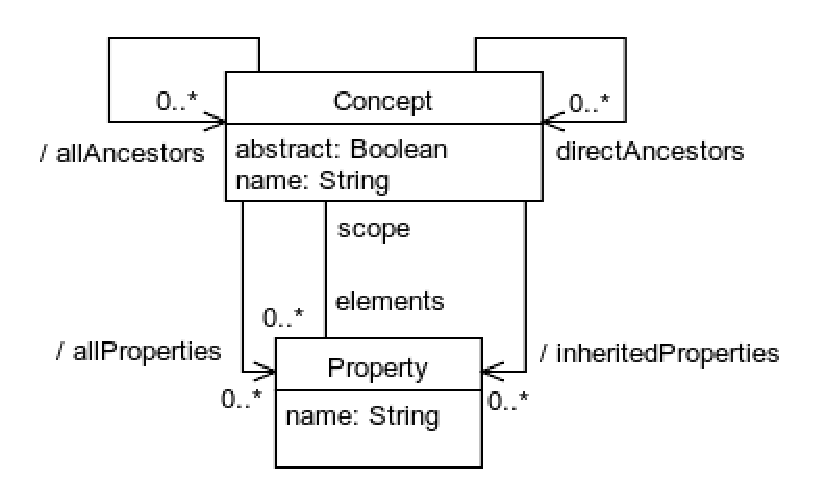
\includegraphics[width=\textwidth]{metamodel/concept}
\caption{Concept Metamodel}
\label{fig:meta:concept}
\end{figure}

\begin{figure}
\verbatimfont{\small}
\begin{framed}
\verbatiminput{ast/concept.lsl}
\end{framed}
\caption{Concept AST Instantiation}
\label{fig:ast:concept}
\end{figure}

\begin{constraints}
Figure \ref{fig:ocl:concept} presents the invariants of the \emph{concept} metamodel:

\begin{itemize}

\item \emph{unique\_concept\_name}:
Each \emph{concept} must have a unique NAME within its \emph{module} (\ref{ch:modules}).

\item \emph{not\_own\_ancestor}:
A \emph{concept} may not be listed on its own \emph{AncestorList},
nor on the \emph{AncestorList} of its direct or indirect ancestors.

\end{itemize}
\end{constraints}

\begin{figure}
\verbatimfont{\small}
\begin{framed}
\verbatiminput{ocl/concept.ocl}
\end{framed}
\caption{Concept Constraints}
\label{fig:ocl:concept}
\end{figure}
